\documentclass[a4paper]{article}
\usepackage[affil-it]{authblk}
\usepackage{listings}
\usepackage{geometry}
\usepackage{amsmath}
\usepackage{amssymb}
\usepackage{graphicx}
\usepackage{float}
\geometry{margin=1.5cm, vmargin={0pt,1cm}}
\setlength{\topmargin}{-1cm}
\setlength{\paperheight}{29.7cm}
\setlength{\textheight}{25.3cm}

\begin{document}

\title{Numerical Analysis Programming Homework 2}
\author{DAVE JOVAN TANDIONO 3210300364 \thanks{Electronic address: minmindjt@gmail.com}}
\affil{Information and Mathematical Science 2101, Zhejiang University}
\date{Due time: October 29, 2024}

\maketitle

\begin{abstract}
This report covers the implementation and analysis of Newton, Hermite, and Bezier interpolation methods. Each section includes brief descriptions of class structure, key functions, and solution discussions for problems B and C, demonstrating Runge's phenomenon and the benefits of Chebyshev interpolation.
\end{abstract}

\section*{Design for Interpolation Methods}

\subsection*{Newton Interpolation}
The \texttt{NewtonInterpolation} class calculates values using Newton’s divided difference formula.
\begin{itemize}
    \item \texttt{computeDividedDifferences()}: Calculates divided differences.
    \item \texttt{interpolate(double x)}: Evaluates the polynomial at \( x \).
\end{itemize}

\begin{lstlisting}
class NewtonInterpolation {
public:
    NewtonInterpolation(const std::vector<double>& x_values, const std::vector<double>& y_values);
    double interpolate(double x) const;
private:
    void computeDividedDifferences();
    std::vector<double> x_values_, y_values_, divided_diffs_;
};
\end{lstlisting}

\subsection*{Hermite Interpolation}
\texttt{HermiteInterpolation} considers both function values and derivatives.
\begin{itemize}
    \item \texttt{computeCoefficients()}: Computes polynomial coefficients.
    \item \texttt{evaluate(double t)}: Evaluates the Hermite polynomial.
    \item \texttt{derivative(double t)}: Finds the derivative, useful for velocity estimation.
\end{itemize}

\begin{lstlisting}
class HermiteInterpolation {
public:
    HermiteInterpolation(const std::vector<double>& x_values, const std::vector<double>& y_values, const std::vector<double>& y_prime_values);
    double evaluate(double t);
    double derivative(double t);
private:
    void computeCoefficients();
};
\end{lstlisting}

\subsection*{Bezier Curve Approximation}
The \texttt{BezierCurve} class approximates complex shapes like a heart using cubic Bezier curves based on Algorithm 2.74.
\begin{itemize}
    \item \texttt{generateHeartBezier(int m)}: Generates Bezier points for the heart shape approximation, varying detail based on \( m \).
    \item \texttt{computeBezierCurve(const std::vector<std::pair<double, double>>\& points, int m)}: Computes control points for each Bezier segment.
\end{itemize}

\begin{lstlisting}
class BezierCurve {
public:
    BezierCurve();
    std::vector<std::pair<double, double>> generateHeartBezier(int m);
private:
    std::pair<double, double> heartFunction(double t);
    std::vector<std::pair<double, double>> computeBezierCurve(
        const std::vector<std::pair<double, double>>& points, int m);
};
\end{lstlisting}

\section*{Problem B: Runge's Function and Polynomial Interpolation}
Newton interpolation was applied to \( f(x) = \frac{1}{1 + x^2} \) on \( x \in [-5, 5] \) using \( x_i = -5 + 10 \frac{i}{i/n} \) with \( n = 2, 4, 6, 8 \). Increasing \( n \) causes oscillations at the edges (Runge phenomenon), as shown in Figure~\ref{fig:runge}.

\begin{figure}[H]
    \centering
    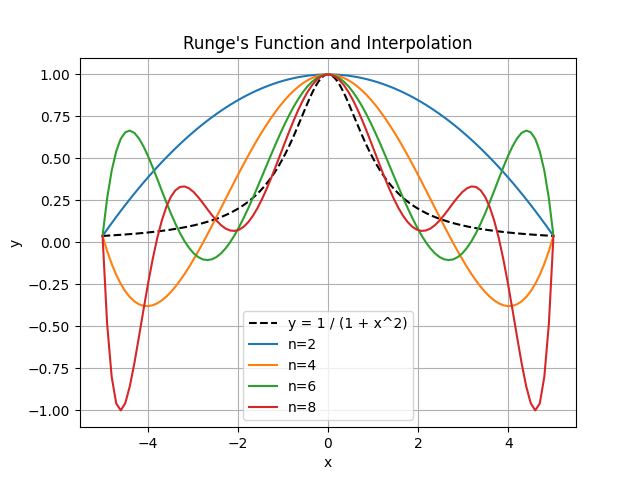
\includegraphics[scale=0.5]{B.png}
    \caption{Runge's Function and Interpolations for \( n = 2, 4, 6, 8 \).}
    \label{fig:runge}
\end{figure}

\section*{Problem C: Chebyshev Interpolation}
Using Newton interpolation with Chebyshev nodes for \( f(x) = \frac{1}{1 + 25x^2} \) over \( x \in [-1, 1] \), we observe reduced oscillations even as \( n \) increases (Figure~\ref{fig:chebyshev}), illustrating the effectiveness of Chebyshev nodes for high-curvature functions.

\begin{figure}[H]
    \centering
    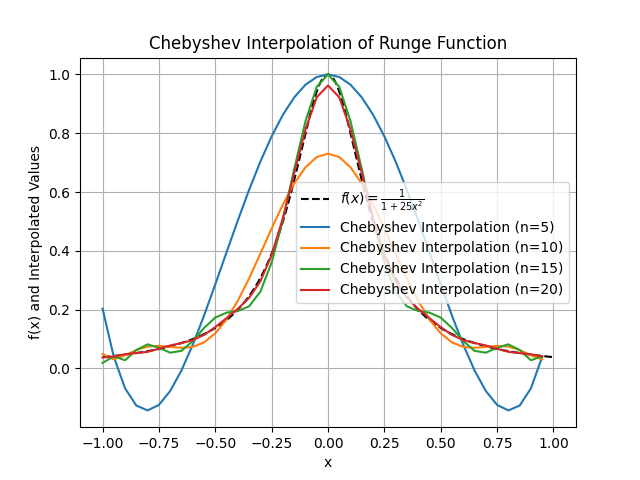
\includegraphics[scale=0.5]{C.png}
    \caption{Chebyshev Interpolation for \( n = 5, 10, 15, 20 \).}
    \label{fig:chebyshev}
\end{figure}

\section*{Problem D: Hermite Interpolation for Car Displacement}
Given displacement and velocity data at different times, Hermite interpolation was used to predict displacement and velocity at \( t = 10 \) seconds. 
Results:
\begin{itemize}
    \item Predicted displacement at \( t = 10 \): 742.503 feet
    \item Predicted velocity at \( t = 10 \): 48.382 feet/second
\end{itemize}
The car does not exceed the speed limit of 81 feet/second, as confirmed by the derivative check at this point.

\section*{Problem E: Average Weight Curve Approximation for Larvae}
For this problem, Hermite interpolation was employed to estimate the average weight of larvae at a specific day (Day 43). Two samples were analyzed:

\begin{itemize}
    \item \textbf{Sample 1 (Young Leaves):} Predicted weight at Day 43 is \(14640.3\) mg.
    \item \textbf{Sample 2 (Mature Leaves):} Predicted weight at Day 43 is \(2981.48\) mg.
\end{itemize}

Based on the predictions:
\begin{itemize}
    \item \textbf{Sample 1 larvae} show signs of survival with a weight of \(14640.3\) mg.
    \item \textbf{Sample 2 larvae} also show signs of survival with a weight of \(2981.48\) mg.
\end{itemize}

These results suggest the viability of both larvae samples under different conditions, with weights indicating growth and development by Day 43. This method allows us to assess potential survival rates and growth trends based on available data points and their derivatives.

\section*{Problem F: Bézier Curve Approximation of Heart Shape}
Three Bézier curves approximating a heart shape were generated for \( m = 10, 40, 160 \) (Figure~\ref{fig:bezier}).
The Bézier method produced increasingly smooth approximations as \( m \) increased, highlighting the method’s effectiveness for approximating curves with high symmetry and continuous changes in curvature.

\begin{figure}[H]
    \centering
    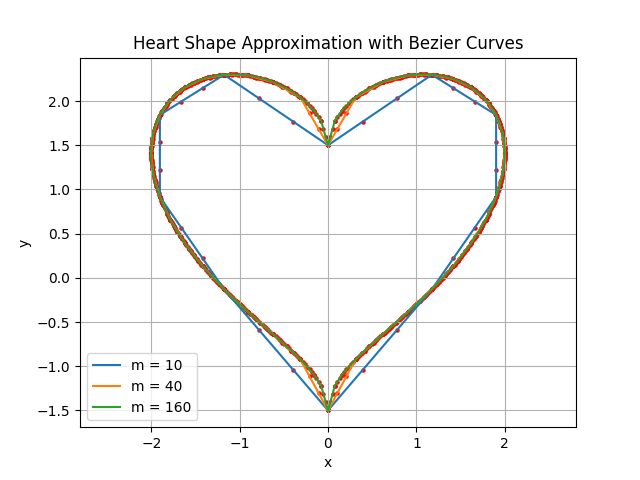
\includegraphics[scale=0.5]{F.png}
    \caption{Heart-shaped Curve Approximations using Bézier Curves for \( m = 10, 40, 160 \).}
    \label{fig:bezier}
\end{figure}

\section*{\center{\normalsize {Acknowledgment}}}
I would like to acknowledge the assistance of ChatGPT, which provided valuable insights and support in understanding the concepts, structuring the solutions, and developing the code for this assignment. 

\end{document}


